\documentclass{article}
    \usepackage{xparse}
    \usepackage[margin=2cm]{geometry}
	\usepackage{enumerate} 
    \usepackage{textcomp}
	\frenchspacing
	\linespread{1.2}

    \usepackage[polish]{babel}
    \usepackage[utf8]{inputenc}
    \usepackage{polski}

	\usepackage{amsthm}
	\usepackage{amsmath}
	\usepackage{amsfonts}
	\usepackage{float}
    \usepackage{diagbox}
	\usepackage{hhline}
	\usepackage{graphicx}
	\usepackage{multirow}
	\usepackage{mathtools}

	\theoremstyle{definition}
	\newtheorem{zadanie}{Zadanie}[subsection]
	\renewcommand{\thezadanie}{\arabic{zadanie}}

\title{\textbf{Query-by-Sketch: Scaling Shortest Path Graph Queries on Very Large Networks}}

\author{Paweł Polerowicz}
\date{Styczeń 2024}

\begin{document}
    \maketitle
    \section{Wiadomości wstępne}
    
    \subsection{Informacje o artykule}
    \begin{itemize}
        \item Tytuł: Query-by-Sketch: Scaling Shortest Path Graph Queries on Very Large Networks
        \item Autorzy: Ye Wang, Qing Wang, Henning Koehler, Yu Lin
        \item Data publikacji: 2021
        \item miejsce publikacji: Proceedings of the 2021 International Conference on Management of Data
    \end{itemize}
    
    \subsection{Słowniczek pojęć}

    \begin{tabular}{|l | l | } 
        \hline
        Oznaczenie & Znaczenie \\
        \hline\hline
        $G(V,E)$ & graf (tu nieskierowany i spójny) \\ 
        \hline
        $P_{uv}$ & zbiór najkrótszych ścieżek między wierzchołkami $u$ i $v$ \\ 
        \hline
        $d_G(u, v)$ & długość najkrótszej ścieżki między $u$ i $v$ \\ 
        \hline
        $R \subset V$ & zbiór punktów orientacyjnych (ang. \textit{Landmarks}) \\ 
        \hline
        $L(v) = \{(r_1, \delta_{vr_1}),\cdots,(r_n, \delta_{vr_n})\}$ & zbiór etykiet wierzchołka $v$ \\ 
        \hline
        $\delta_{vr_i}$ & $= d_G(v, r_i)$ \\ 
        \hline
        $L = \{L(v)\}_{v \in V}$ & etykietowanie nad $G$\\ 
        \hline
        $size(L) = \sum_{v \in V}|L(v)|$ & rozmiar etykietowania \\ 
        \hline
    \end{tabular}\\
    
    \subsection{Plan prezentacji}
        W ramach niniejszej prezentacji zreferujemy artykuł \textit{Query-by-Sketch: Scaling Shortest Path Graph Queries on Very Large Networks}, przedstawiający metodę QbS. Składa się ona z trzech algorytmów. Pierwszy z nich służy jako przetwarzanie wstępne i są wykonywany raz i wyznacza etykietowanie $L$ dla grafu $G$. Drugi tworzy szkic danych dla pary wierzchołków $u$ i $v$ na podstawie etykietowania $L$. Ostatni wyznacza dokładną odpowiedź, wykorzystując przeszukiwanie kierowane szkicem. Złożoności algorytmów to kolejno $O(|R||E|)$, $O(|R|^4)$ (z możliwością ograniczenia do $O(|R|^2)$) oraz $O(|E| + |R||V|)$, gdzie R jest zbiorem punktów orientacyjnych.

    \subsection{Motywacja}
        Podczas poprzednich prezentacji omawialiśmy struktury wykorzystujące szkice danych do efektywnego pamięciowo przechowywania informacji o strumieniowanym grafie. W szczególności rozważaliśmy takie konstrukcje, które pozwalały na uzyskiwanie szybkich odpowiedzi na zapytania o istnienie i wagę krawędzi między dwoma wierzchołkami, a także łączną wagę krawędzi wchodzących i wychodzących z danego wierzchołka. Niemniej jednak często zależy nam na wykonywaniu bardziej skomplikowanych operacji. Jedną z typowych może być wyznaczanie najkrótszych ścieżek między wierzchołkami. Rozwiązania tego problemu mogą znaleźć swoje zastosowanie np. w nawigacji GPS lub w analizie sieci społecznościowych. W obu przypadkach mamy do czynienia z grafami o nierzadko ogromnych rozmiarach. Sprawia to, że klasyczne i dobrze przebadane algorytmy mogą okazać się nieskuteczne, ze względu na konieczność przeglądu zatrważającej liczby krawędzi lub wykorzystywania dodatkowej pamięci o niepraktycznym rozmiarze. Dodatkowo niejednokrotnie możemy być zainteresowani wyborem nie jednej ścieżki, lecz pewnego zbioru najkrótszych lub prawie najkrótszych ścieżek. Śledząc wysiłki autorów artykułu, spróbujemy znaleźć metodę wyznaczania grafu najkrótszych ścieżek w sposób wydajny czasowo i przy użyciu rozsądnej ilości pamięci. 
    
    \section{Problem}
    
    \subsection{Sformułowanie problemu}

        \subsubsection*{2-hop distance cover (dwu-przeskokowe pokrycie odległości :))}
            Etykietowanie $L$ grafu $G$ stanowi 2-hop distance cover, jeśli zachodzi 
            \[
                \forall_{u,v \in V} d_G(u, v) = min\{\delta_{ur} + \delta_{vr} : (r, \delta_{ur}) \in L(u), \delta_{vr} \in L(v)\}    
            \]
            Innymi słowy, wymagamy, aby dla każdej pary wierzchołków, ich etykiety zawierały co najmniej jeden wspólny punkt orientacyjny leżący na jednej z najkrótszych ścieżek je łączących. 
    
        \subsubsection*{SPG (graf najkrótszych ścieżek)}
            Dla dowolnych dwóch wierzchołków $u$ i $v$, graf najkrótszych ścieżek (SPG) między $u$ i $v$ to podgraf $G_{uv}$ grafu, gdzie:
            \begin{enumerate}
                \item $V(G_{uv}) = \bigcup_{p \in P_{uv}} V(p)$
                \item $E(G_{uv}) = \bigcup_{p \in P_{uv}} E(p)$
            \end{enumerate}
            Graf ten nie jest więc po prostu podgrafem indukowanym przez $\bigcup_{p \in P_{uv}} V(p)$, gdzie $P_{uv}$ to zbiór najkrótszych ścieżek między wierzchołkami $u$ i $v$. Każda jego krawędź musi być bowiem częścią najkrótszej ścieżki między $u$ i $v$. 

        \subsubsection*{Problem SPG}
            Niech $G = (V, E)$ oraz $u,v \in V$. Problem SPG polega na znalezieniu odpowiedzi na zapytanie $SPG(u,v)$, czyli grafu najkrótszych ścieżek $G_{uv}$ dla $G$. W niniejszej prezentacji będziemy dla uproszczenia zakładali, że graf jest nieskierowany, spójny i nie jest ważony. W ogólności jednak te ograniczenia są możliwe do zrelaksowania. 
            
    \subsection{Główne idee rozwiązań}

    \section{Przegląd poprzednich rozwiązań}
        
    \subsection{Klasyczne algorytmy}

        \subsection{Algorytmy dokładne dla dużych grafów}

        \subsection{Algorytmy aproksymacyjne}

            
    \section{QbS}
    
    \subsection{Idea}

    \begin{figure}[!tbh]
        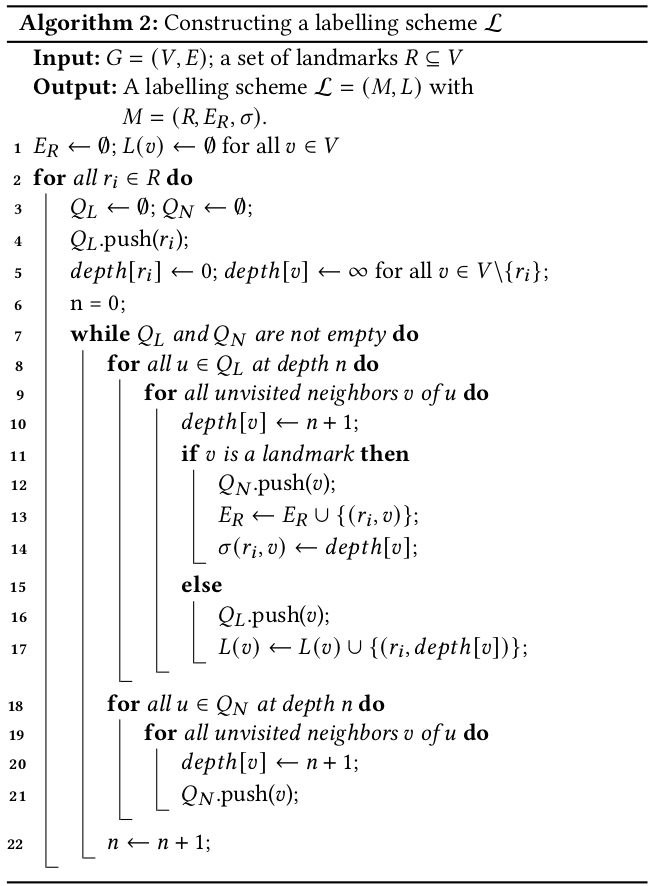
\includegraphics[width=11cm]{img/algorithm_2.png}
        \centering
        \label{fig:alg2}
        \caption{Pseudokod procedury etykietowania}
    \end{figure}


    \begin{figure}[!tbh]
        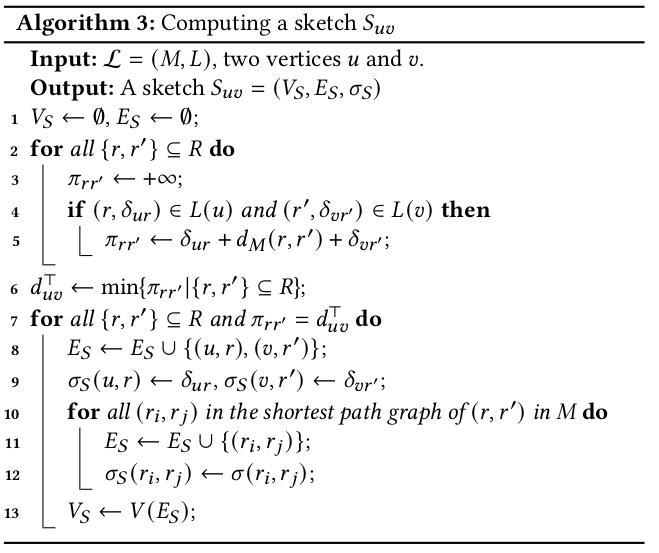
\includegraphics[width=11cm]{img/algorithm_3.png}
        \centering
        \label{fig:alg3}
        \caption{Pseudokod procedury szkicowania}
    \end{figure}


    \begin{figure}[!tbh]
        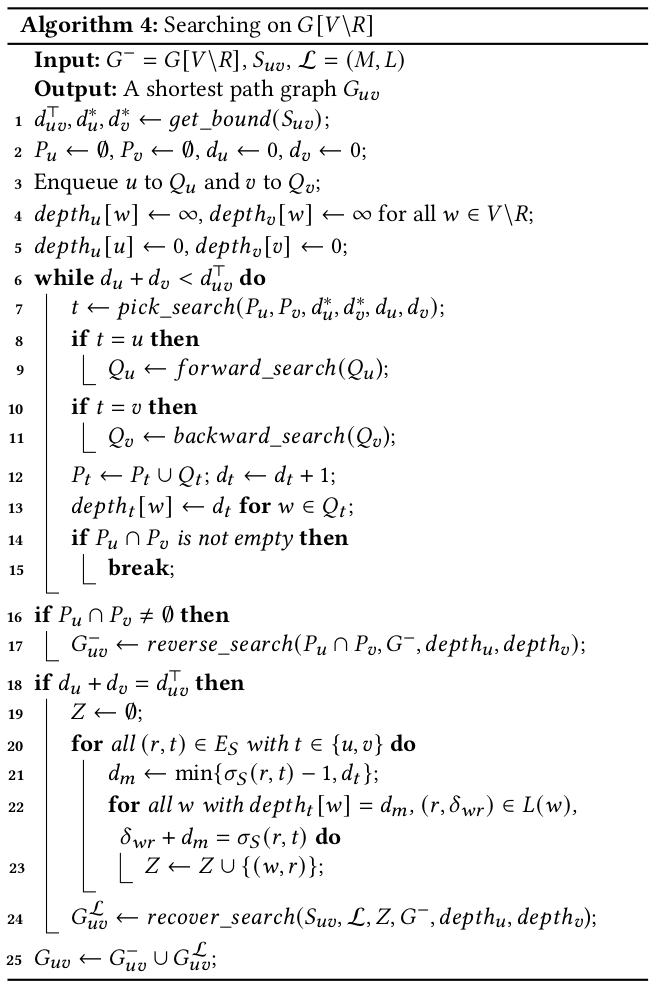
\includegraphics[width=11cm]{img/algorithm_4.png}
        \centering
        \label{fig:alg4}
        \caption{Pseudokod przeszukiwania kierowanego szkicem}
    \end{figure}

    \subsection{Przykład}
     
    \subsection{Etykietowanie}

    \subsection{Szkicowanie grafu najkrótszych ścieżek}

    \subsection{Przeszukiwanie kierowane}
        
    \subsection{Poprawność}

    \subsection{Złożoność pamięciowa}
    
    \subsection{Złożoność czasowa (szkic)}

    \subsection{Urównoleglenie}
    

    \subsection{Zależność od liczby punktów orientacyjnych}
    
    \section{Zakończenie}
    Dziękuję słuchaczom za uwagę i życzę miłego dnia. 
    
\end{document}